\begin{figure*}[t]
  \centering
  \begin{tabular}{@{}cccc@{}}
    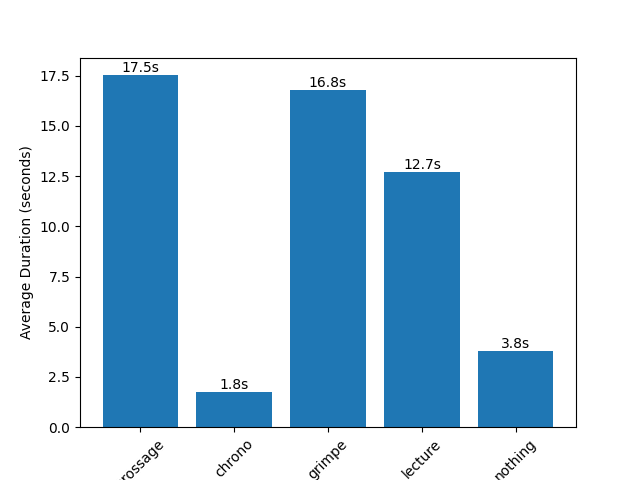
\includegraphics[width=0.23\textwidth]{../../assets/figures/average-duration-of-actions.png} &
    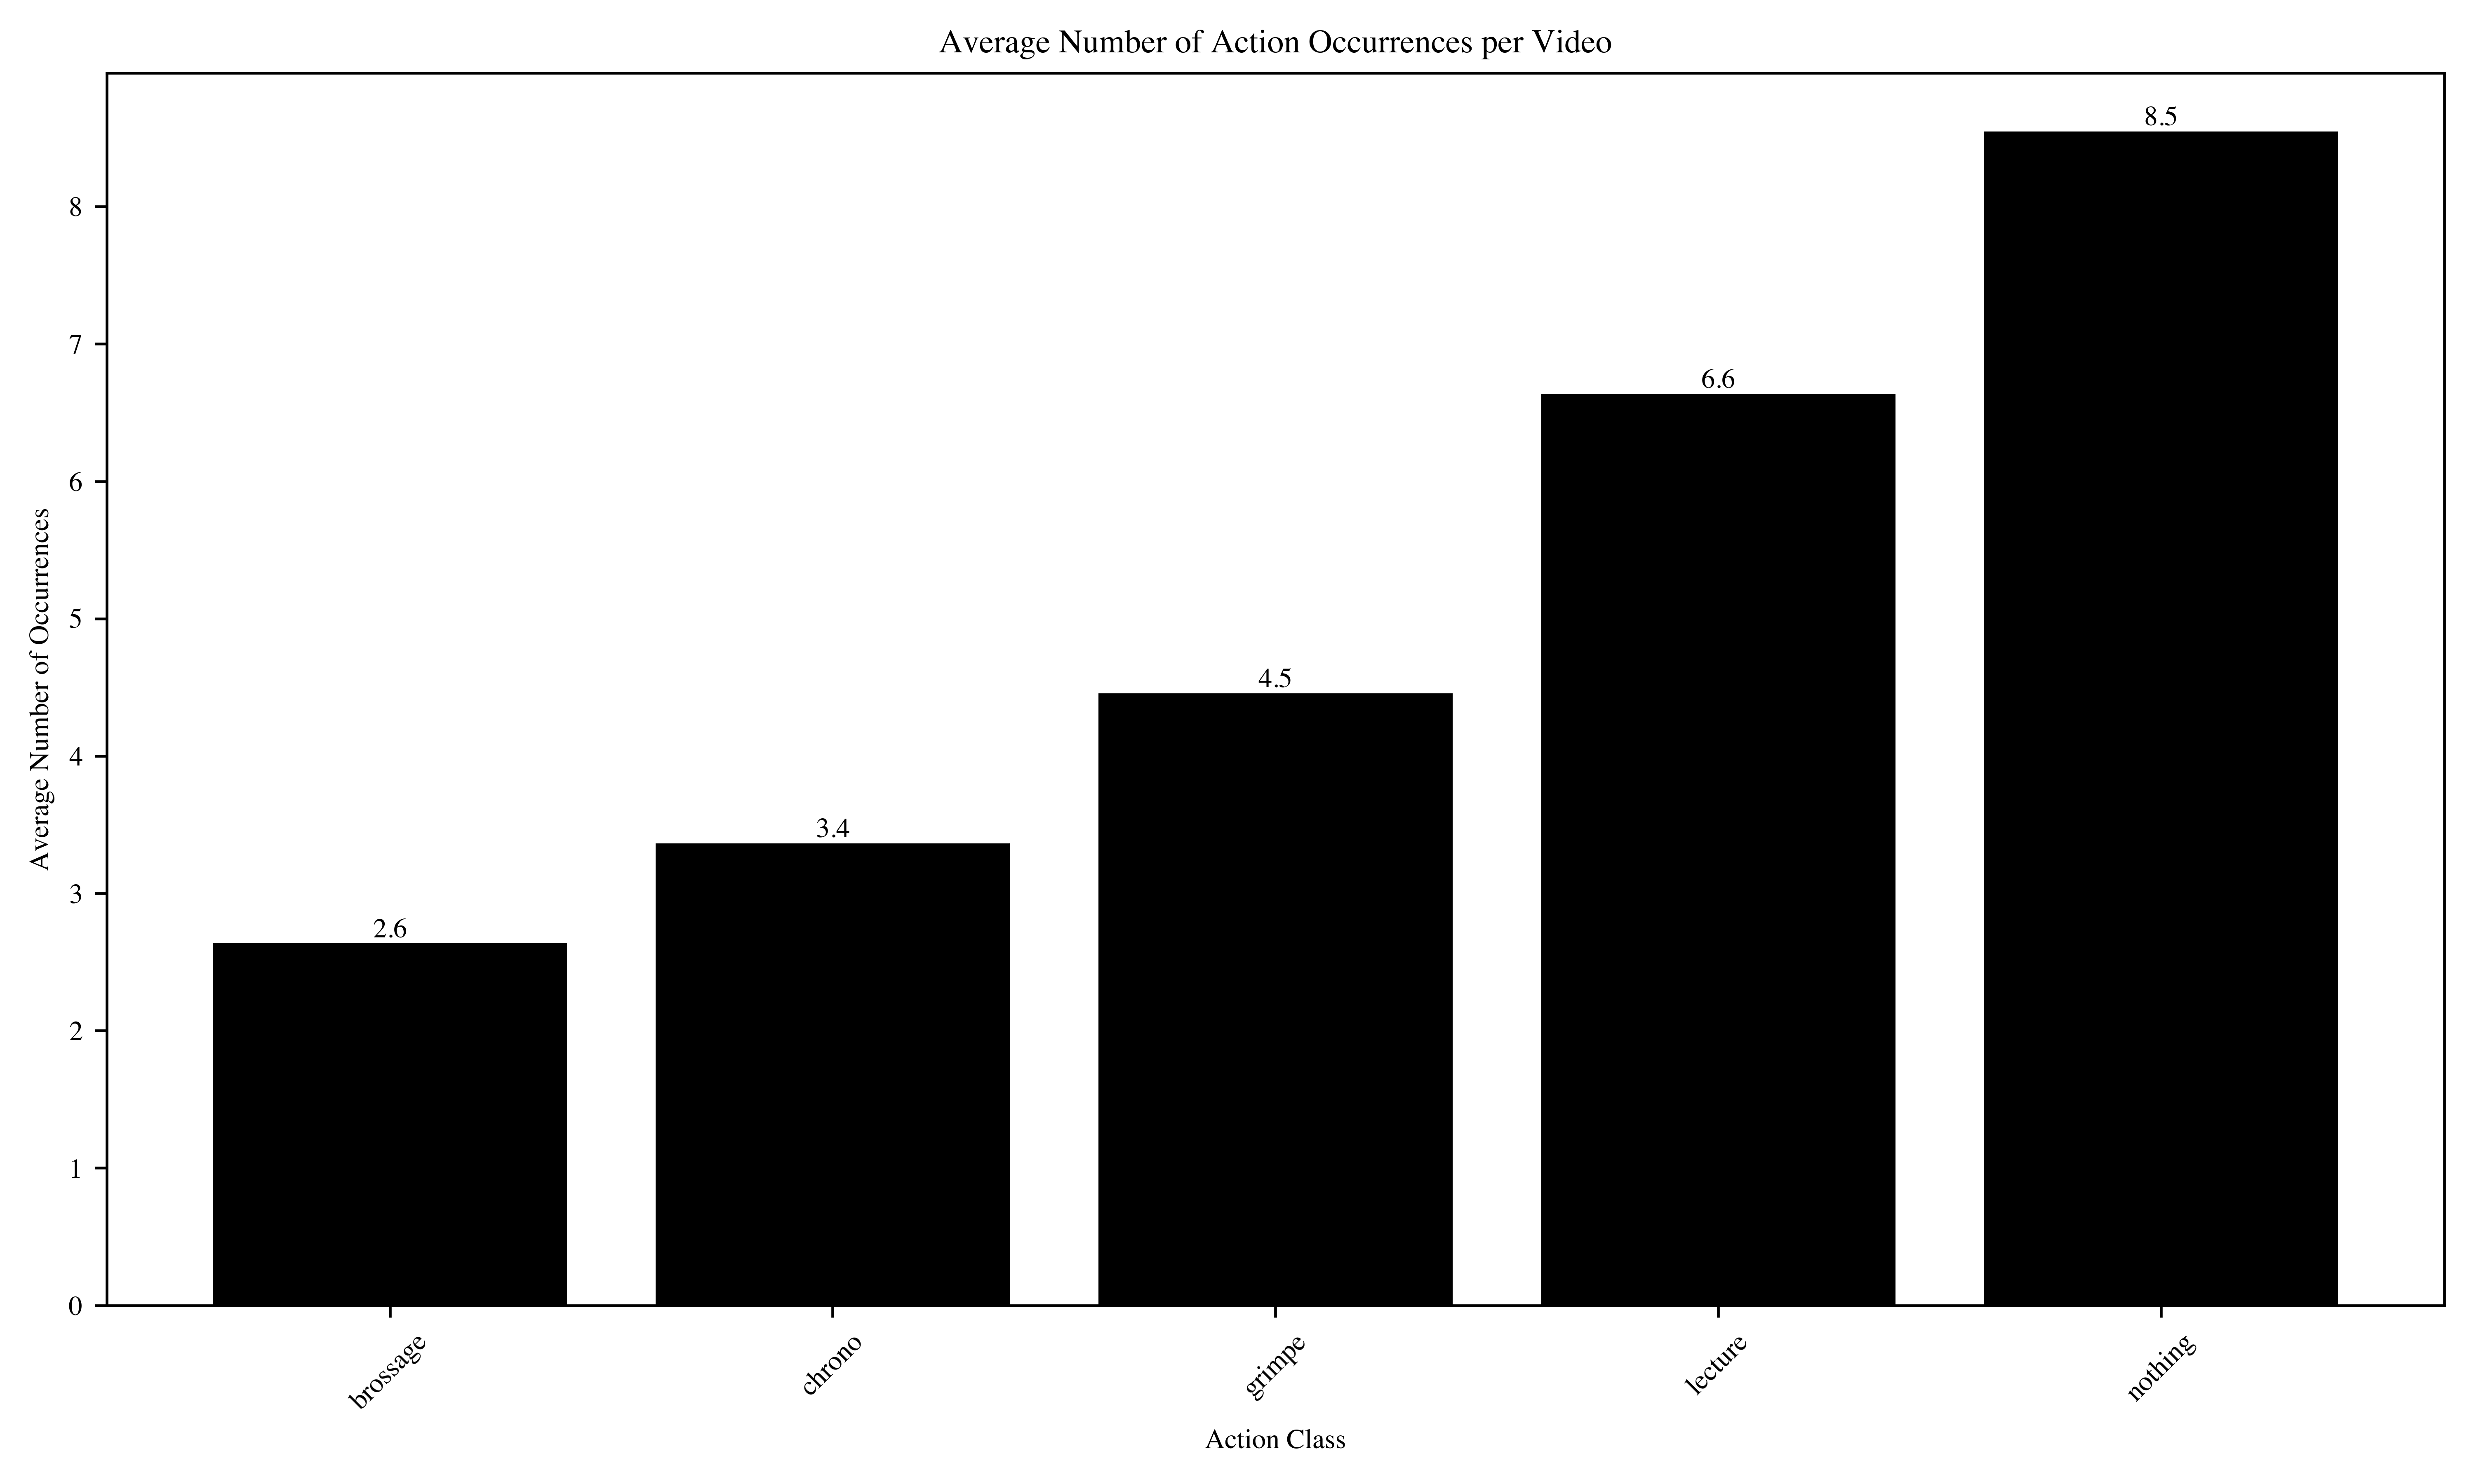
\includegraphics[width=0.23\textwidth]{../../assets/figures/average-number-of-action-occurrences-per-video.png} &
    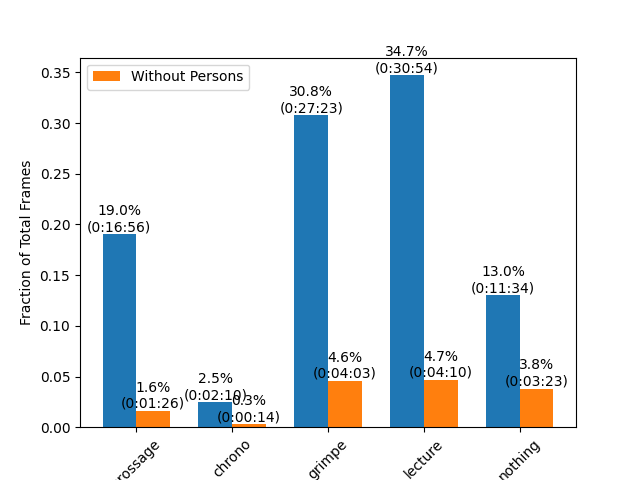
\includegraphics[width=0.23\textwidth]{../../assets/figures/distribution-of-actions-in-dataset.png} &
    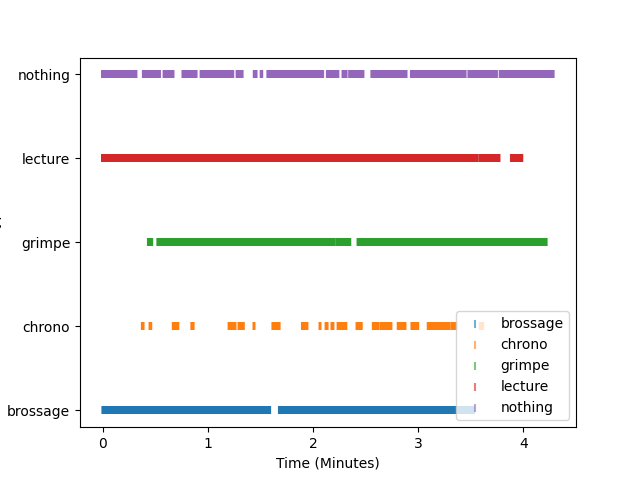
\includegraphics[width=0.23\textwidth]{../../assets/figures/temporal-distribution-of-actions.png} \\
    \begin{minipage}{0.23\textwidth}\centering\caption{Average duration of actions in the dataset.}\label{fig:average-duration-of-actions}\end{minipage} &
    \begin{minipage}{0.23\textwidth}\centering\caption{Average Action Count per Video.}\label{fig:average-number-of-action-occurences-per-video}\end{minipage} &
    \begin{minipage}{0.23\textwidth}\centering\caption{Distribution of actions in the dataset.}\label{fig:distribution-of-actions-in-dataset}\end{minipage} &
    \begin{minipage}{0.23\textwidth}\centering\caption{Temporal distribution of actions in the dataset}\label{fig:temporal-distribution-of-actions}\end{minipage}
  \end{tabular}
\end{figure*}

\section{Dataset}

In this section, we present the dataset used in this project, detailing its construction, preparation, and some important statistics. We also compare our dataset to other popular datasets used in temporal action segmentation.

\subsection{Raw Format}

Our dataset was collected during the "Manip Chambery" bouldering event. It consists of videos filmed from two different angles of 10 climbers attempting to complete 2 distinct bouldering blocks (events) each. This resulted in a total of 20 unique climbs, or 40 videos in total, with each video having a duration of 4 minutes.

The climbers' activities during the event are diverse. They may engage in actions such as brushing the holds, observing them, and climbing. These actions occur freely within the 4-minute duration of each video, providing a rich set of diverse activities.

As specified in \cite{section:context}, the videos were annotated by the climbers themselves, and the annotations were provided in raw Excel format. The annotations are segment-level, meaning that for each action, we are given the start time and duration of the activity, along with the corresponding label. Out of the 20 climbs, 11 have been annotated with action segments.

The total duration of the dataset is 2 hours and 40 minutes, of which 1 hour and 28 minutes are annotated, forming the basis of our experiments.

\noindent\textbf{Dataset Limitations.}  
While the dataset provides valuable data for action segmentation tasks, it has several limitations: 

\textbf{1.} The dataset size is relatively small, containing only 40 unique videos.
\textbf{2.} The annotations are provided in Excel format, which is not ideal for modern data science workflows.
\textbf{3.} The annotations themselves are not perfect, as they may be shifted in time, and the videos do not always start precisely at the beginning of the event.
\textbf{4.} Climbers occasionally leave the frame during the video, and in some instances, other people may enter the frame, which introduces noise to the data.
\textbf{5.} The dataset includes a 'nothing' class, representing periods with no relevant activity, which can further imbalance the dataset and affect model performance.  

Despite these limitations, this dataset provides an essential foundation for the development and evaluation of action segmentation models in the context of bouldering.
\subsection{Chosen Structure}

We decided to structure the dataset in a way that is specifically suited for temporal action segmentation and classification tasks, with a focus on both ease of use and efficiency for training. This structure is designed to allow for easy scalability as new data is added to the project, an important consideration as the dataset will be updated by individuals who may not have a background in data science.

\begin{verbatim}
    dataset
    +-- videos
    |   +-- video-1
    |   |   +-- frame-1.jpg
    |   |   +-- frame-2.jpg
    |   |   +-- ...
    |   +-- ...
    +-- annotations
    |   +-- video-1.csv
    |   +-- video-2.csv
    |   +-- ...
\end{verbatim}

The advantage of this structure is that it does not require additional processing of the videos or annotations provided by the data collection team, ensuring the dataset can be easily expanded with new annotations or videos in the future.

To optimize for video loading, we store each video as a sequence of JPG frames rather than the video file itself. This avoids the need for decoding during runtime, though it comes at the cost of additional storage space. This structure also makes the dataset more versatile and compatible with various libraries and tools.

\begin{AIbox}{Python Package - Video Dataset.}
  We have developed a Python package, \href{https://github.com/raideno/video-dataset}{https://github.com/raideno/video-dataset}, to support this dataset structure. The package provides utilities for easily loading videos, transforming them into this frame-based format, and handling annotations at the frame level. It is highly customizable and can be adapted to work with different types of datasets.
\end{AIbox}

A related tool, \href{https://github.com/raideno/cached-dataset}{https://github.com/raideno/cached-dataset}, serves as a wrapper for an existing dataset, caching the transformed version on disk. This is particularly useful in avoiding the need to repeatedly extract features during model training or evaluation. We will discuss the details of this tool in the training procedure section.

By utilizing this structure and the provided tools, we were able to quickly load the dataset and begin training the model.

\subsection{Data Exploration}  
In this section, we explore key aspects of our bouldering dataset to better understand its characteristics and potential challenges for model training.

\begin{table}[!h]
\centering
\small

\resizebox{1\linewidth}{!}{
\begin{tabular}{ccc}
\toprule
Imbalance Ratio & Average Repetition Score & Order Variation Score \\
\midrule
14.16 & 0.81 ± 0.04 & 0.49 \\
\bottomrule
\end{tabular}
}
\vspace{-2ex}\caption{Dataset statistics}
\label{table:dataset-statistics}
\end{table}


As shown in Figure \ref{fig:distribution-of-actions-in-dataset}, our dataset contains five action classes: cleaning ("brossage"), climbing ("grimpe"), observation ("lecture"), nothing, and break ("chrono"). The distribution is notably unbalanced, with "lecture" being the most frequent at 34.7\%, followed by "grimpe" at 30.8\%. The cleaning action ("brossage") represents 19.0\%, while "chrono" accounts for only 2.5\%. This imbalance is reflected in the dataset's imbalance ratio of \textbf{14.16}, indicating a significant risk of the model overfitting to the dominant classes.

Figure \ref{fig:temporal-distribution-of-actions} reveals that "grimpe" is less common at the beginning of videos, aligning with climbers preparing their attempts through cleaning or observation. Conversely, "lecture" and "brossage" actions are rare at the end of videos, suggesting that climbers tend to finalize their attempts rather than engage in preparation during these moments. This temporal pattern highlights the importance of incorporating time-dependent features in our model.

From Figure \ref{fig:average-number-of-action-occurences-per-video}, we observe that "nothing" appears most frequently, averaging 8.5 instances per video. While this class is important for capturing pauses and transitions, its dominance risks overwhelming the model if not carefully balanced. Additionally, the low frequency of "chrono" (3.4 occurrences per video) may challenge the model's ability to accurately detect this class.

Figure \ref{fig:average-duration-of-actions} highlights further complexities: "brossage" has the longest average duration at 17.5 seconds, while "chrono" has the shortest at just 1.9 seconds. The brief duration of "chrono," combined with its low frequency, makes it particularly vulnerable to misclassification.

Lastly, the dataset's \textbf{average repetition score of 0.81} suggests a high degree of repetitive patterns in action sequences, which may lead the model to exploit these patterns rather than learning meaningful action transitions. Additionally, the \textbf{order variation score of 0.49} reveals some variability in action order, which may require the model to adapt to less predictable sequences.

In addition to these challenges, approximately 15\% of the frames contain no visible person, and 3\% include multiple people, introducing further noise. Moreover, 13\% of climbs lack proper annotations and are labeled as "nothing" by default.

These insights highlight key challenges for our model: class imbalance, varying action durations, repetitive patterns, and noisy data. Addressing these issues will be crucial for achieving robust action segmentation performance.

\subsection{Popular Video Datasets}

\label{subsection:popular-video-datasets}

\begin{figure}[h!]
    \centering
    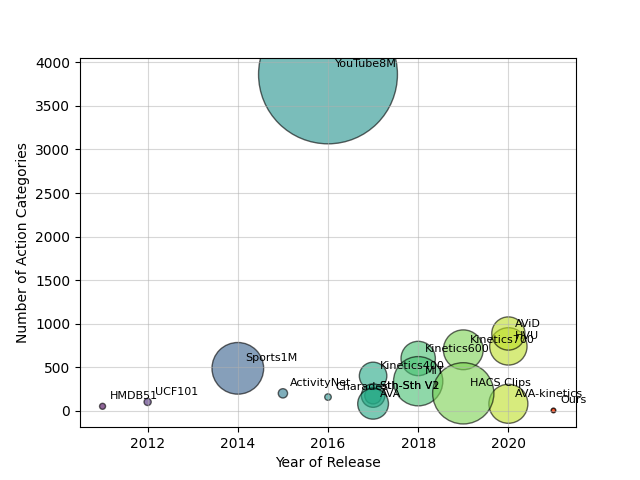
\includegraphics[width=1\linewidth]{../../assets/figures/popular-datasets.png}
    \caption{A visualization of popular video datasets.}
    \label{fig:your-label}
\end{figure}

While there are a number of video datasets available for action recognition and segmentation tasks, the overall number remains limited compared to image or text datasets. Video datasets are much more complex due to the added temporal dimension, and therefore require a significantly larger number of samples for effective model training. For instance, while image datasets might need millions of samples, video datasets typically require tens of millions of samples due to the increased complexity.

Some of the most notable video datasets designed for temporal action segmentation include:

\noindent\textbf{50 Salads Dataset.} This dataset features videos of people preparing salads, focusing on fine-grained hand interactions with the environment \cite{50salads-dataset}.

\noindent\textbf{GTEA Dataset.} Consists of Point of View (POV) videos of food preparation, capturing various sub-actions \cite{gtea-dataset}.

\noindent\textbf{Breakfasts Dataset.} Videos of breakfast preparation, with a focus on fine-grained action segmentation \cite{breakfast-dataset}.

\noindent\textbf{Kinetics Family.} Large-scale datasets containing YouTube clips of various human actions, ranging from sports to human-object interactions \cite{kinetics-400-dataset}, \cite{kinetics-600-dataset}, \cite{kinetics-700-dataset}.

\noindent\textbf{Assembly101 Dataset.} Videos of people assembling and disassembling objects, captured from multiple angles, including some POV \cite{assembly101-dataset}.

\noindent\textbf{HowTo100M Dataset.} A massive dataset of instructional (tutorial) videos, covering a broad range of activities \cite{howto100m-dataset}.

\noindent\textbf{Something-Something V2.} Videos of basic actions such as picking up a pen, captured from a POV perspective, focusing on fine-grained interactions \cite{something-something-dataset}.

Note that the three first datasets were specifically designed for temporal action segmentation.

\begin{table}[!h]
    \centering
    \small
    \resizebox{1\linewidth}{!}{
    \begin{tabular}{lcrr}
    \toprule
    Dataset & Release Year & \#Samples & \#Actions \\
    \midrule
    HMDB51 & 2011 & 7000 & 51 \\
    UCF101 & 2012 & 13300 & 101 \\
    Sports1M & 2014 & 1100000 & 487 \\
    ActivityNet & 2015 & 28000 & 200 \\
    YouTube8M & 2016 & 8000000 & 3862 \\
    AVA & 2017 & 385000 & 80 \\
    \multicolumn{1}{c}{\vdots} & \multicolumn{1}{c}{\vdots} & \multicolumn{1}{c}{\vdots} & \multicolumn{1}{c}{\vdots} \\
    MIT & 2018 & 1000000 & 339 \\
    HACS Clips & 2019 & 1550000 & 200 \\
    HVU & 2020 & 572000 & 739 \\
    AViD & 2020 & 450000 & 887 \\
    \midrule
    \textbf{Ours} & 2024 & 22 & 4 \\
    \bottomrule
    \end{tabular}
    }
    \vspace{-2ex}\caption{A list of popular video datasets.}
    \end{table}